\documentclass[
    bindingoffset=5mm,  % Binding offset
    footnoteindent=3mm, % Footnote indent
    hyphenation=true    % Hyphenation turn on/off
]{tpl/wut-thesis}

\addbibresource{bibliography.bib}
\DeclareBibliographyCategory{commit}

\EngineerThesis
\langeng

\begin{document}

%------------------
% Title page
%------------------
\institute{Telecommunications}
\fieldofstudy{Telekomunikacja}
\specialization{Teleinformatyka i Zarządzanie w Telekomunikacji}
\title{
  Notipie -- notification aggregator
}
% Polish title
\poltitle{
  Notipie -- agregator powiadomień
}
\author{Błażej Sewera}
\studentnumber{300499}
\supervisor{Maciej Sosnowski, M.Sc.}
\date{2022}
\maketitle

%-------------------------------------
% English abstract
%-------------------------------------
\cleardoublepage % Starting from an odd page
\abstract
Notipie is a notification system,
ultimately aiming at unifying
different notification standards,
providing its users with a single source of truth
for their notifications,
and eliminating the need
for the troublesome e-mail notifications.
The overall goal of this project
was to create a full-stack application
that can present the notifications to the user
with a web-based graphical user interface,
and a library
for simple notification creation.
The challenges this project posed include,
inter alia,
the use of the latest web technologies,
deep understanding of~backend development in Go language,
and project management.

\keywords notifications, web application, full-stack


%----------------------------------------
% Polish abstract
%----------------------------------------
\clearpage
\secondabstract
Notipie to system powiadomień,
mający na celu ujednolicenie
różnych standardów powiadomień.
Zapewnia on użytkownikowi
jedno uniwersalne miejsce
do przeglądania powiadomień,
oraz uwalnia użytkownika od korzystania
z uciążliwych powiadomień mailowych.
Głównym celem tego projektu
było stworzenie aplikacji sieciowej pełnego stosu,
która po otrzymaniu powiadomienia,
zaprezentuje je użytkownikowi
przy użyciu graficznego interfejsu przeglądarkowego.
Trudności napotkane podczas tego projektu
to, m.in. użycie najnowszych technologii sieciowych,
głębokie zrozumienie programowania w języku Go
oraz zarządzanie projektem.

\secondkeywords powiadomienia, aplikacja sieciowa, pełny stos

\pagestyle{plain}

%----------------------------------------
% Dedication in an unofficial version
% TODO: uncomment when rendering an unofficial version
%----------------------------------------
% \newenvironment{dedication}{
  \clearpage
  \thispagestyle{empty}
  \vspace*{\stretch{1}}
  \itshape
  \raggedright
  \begin{quote}
    }{
  \end{quote}
  \par
  \vspace{\stretch{3}}
  \clearpage
}

\begin{dedication}
  To all the people who told me\\
  to get to work when I needed it,\\
  critiqued me in what I could improve,\\
  made me coffee, tea, food,\\
  and generally made me a happier person.

  \vspace*{\baselineskip}
  Anything I am now proud of\\
  would not be possible without your support.

  \vspace*{\baselineskip}
  Thank you.

  \vspace*{\baselineskip}
  --- Błażej
\end{dedication}


%--------------
% Table of Contents
%--------------
\cleardoublepage
% Limit the depth to 3 levels:
% section, subsection, and subsubsection
\setcounter{tocdepth}{2}
\tableofcontents

%------------
% Sections
%------------
\cleardoublepage
\pagestyle{headings}

% Always start a section from a new page

\clearpage
\section{Introduction}\label{sec:introduction}

We get notifications every day.
Unfortunately,
those notifications either arrive
to our e-mail inboxes,
or worse,
we have to manually check
each and every website an event may have occurred on.

I personally use \ac{CI} -- \ac{CD} pipelines
on Github Actions for my private projects,
and Jenkins for work.
I get loads of e-mail notifications from Icinga.
I check production servers' state on Grafana,
which also sends notifications
for severe events to my work Microsoft Teams.
I check the health of the services
running on my private server\footnote{
  An example of this particular use case
  is presented in appendix~\ref{apx:sample-systemd-service-with-notipie-hooks}.
} with a custom shell script.
The number of notifications I get every day
is usually too big to wrap my head around,
let alone the fact,
that they come from at least five different sources.

Notipie is a response to this problem.
It is specifically designed
to handle custom sources of notifications,
provide easy setup,
good performance,
and a simple interface.
The project's source code can be found
on Github: \url{https://github.com/blazejsewera/notipie}.

In this thesis,
I will demonstrate my solution
by first explaining the problem domain in detail,
and providing necessary definitions.
I will then quickly go through
the project management
to show how this project was conducted,
as well as which tools and practices
I used to achieve my goal.
The next section
will outline the process of implementing
each component in the system,
describe the protocol for communication
between those components,
and talk about the programming practices I used.
I will then describe how I ensured
a good product quality,
and my approach to testing.
After that,
I will lay out the takeaways from the development
of this project.
I will show what went right
and what I wish I had done differently.

\subsection{Existing Solutions}\label{sec:existing-solutions}

There are many solutions
for systems monitoring,
there are e-mail filters
and smart directories.
Most modern operating systems have some kind of a notification center.
So why did I make Notipie in the first place?

First of all,
I needed something \emph{simple}.
I didn't want the hassle of setting up
the whole Grafana stack for my simple use case,
I also didn't want to go through the trouble
of setting an e-mail gate
for my server events and health checks.
I~also~considered IFTTT,
but the pricing~\cite{ifttt_plans_2022}
was too much for my simple usage,
and the built-in integrations
were not suited for my notification needs.

When I thought about easy-to-use,
standardized ways of displaying notifications,
I immediately looked at
the notification systems on smartphones.
Android and iOS have very simple,
yet very usable notifications,
that all go into a single place.
I wanted to have similar behavior
for my custom use cases,
without the need to~install any apps
from the Apple AppStore,
or Google Play Store.



\clearpage
\section{Domain}\label{sec:domain}

\Ac{DDD} is a software design approach
that aligns the code with the reality
of the problem domain.
It achieves said alignment by focusing
on the following components of the problem domain:
its terminology,
the core reasons behind why the software is being developed,
and success definition.
Because of this alignment,
adding new features is easy,
and the understanding of the problem domain
stays in sync with the production code~\cite{millett_patterns_2015}.
A model of the solution is called the domain model.
The production code needs to directly reflect the domain model,
which means that \iac{UL}, a set of definitions
understandable both to domain experts
and to developers~\cite{evans_domain-driven_2003,millett_patterns_2015},
has to be defined.
\Ac{UL} helps with confronting the proposed solutions
between these two groups.

I started tackling the problem domain by
laying out the high-level definitions
of all significant parts
that are necessary to implement the solution.
I wanted the domain of my application
to be as simple and clear as possible.
Therefore,
I came up with \iac{UL}
and defined four main components: Notification, Tag, App, and User.

\subsection{Notification}\label{sec:notification}

The core of the application.
This is the structure
acting as a protocol of communication
between all components in the application domain.
It consists of the text fields,
like title, optional subtitle, optional body,
\acp{URI} for marking the Notification read,
but also an App\footnote{
  The app component is explained in detail in section~\ref{sec:app}
} of origin.

For the distributed nature of the components,
the Notification is always passed by value.
Having an immutable copy of the Notification object
in every place ensures
no unexpected states in the application.
It is easily achieved
using the features of
the Go language\footnote{
  More on Go features in section~\ref{sec:the-benefits-of-using-go}
}.

\subsection{Tag}\label{sec:tag}

The Tag in the Notipie domain
is a Notification broker
between the Apps and the Users.
It stores which Apps are attached
and which Users are subscribed to it.
It also ensures thread-safety
for attaching and detaching of Apps,
as well as subscribing and unsubscribing of Users.

At first,
I wanted it to be named ``Room'',
like a chat room,
so that many Users could have been
in different Rooms,
similar to subscribing to multiple Tags.
However,
it was less understood by people I spoke with,
mainly due to the fact,
that one App sending to different rooms,
and a User being in different rooms simultaneously,
contradicts the existing understanding of chat rooms.

A User can subscribe to the Tag,
and an App can add itself to a Tag.
When that happens,
the forwarding of Notifications
between said App and User is enabled.
Thread-safety of those operations
are ensured by mutexes\footnote{
  A mutual exclusion lock.
  A mutex serializes the execution
  of multiple threads~\cite{mattson_patterns_2004}.
}.
The Tag is actively listening
on the Notification channel (\texttt{NotificationChan}),
and every time a new Notification arrives,
the \texttt{broadcast} method~(listing~\ref{lst:broadcast-method-in-tag})
is executed.
The \texttt{broadcast} method then sends that Notification
to every User subscribed to this Tag.
The flow is presented in figure~\ref{fig:notification-flowchart}.

\begin{figure}[h]
  \centering
  \includegraphics[width=10cm,keepaspectratio]{chart/out/notification-flowchart.pdf}
  \caption{Notification flow in \texttt{domain}}
  \label{fig:notification-flowchart}
\end{figure}

\subsubsection{Technicalities}\label{sec:tag-technicalities}

There is an obvious problem with this approach.
When a User is subscribed to two Tags,
and one App has those two Tags assigned,
then that User can get the same Notification twice
(figure~\ref{fig:duplicated-notification}).
There are two solutions I could think of.

\begin{figure}[h]
  \centering
  \includegraphics[width=10cm,keepaspectratio]{chart/out/duplicated-notification.pdf}
  \caption{Duplicated Notification flow}
  \label{fig:duplicated-notification}
\end{figure}

\paragraph*{Solution 1}\label{par:duplication-solution-1}

This solution assumes the following:

There is a new component in the domain, Router.
It is a centralized component
that knows which App is connected to which Tag,
and which User is subscribed to those Tags
(figure~\ref{fig:notification-router}).

\begin{figure}[h]
  \centering
  \includegraphics[width=15.5cm,keepaspectratio]{chart/out/notification-router.pdf}
  \caption{Notification Router}
  \label{fig:notification-router}
\end{figure}

With this approach,
the User component is simpler,
as it does not need any deduplication logic.
However, there is a whole new component
in the domain, which introduces complexity.
Furthermore, the Router has to be
a Singleton~\cite{gamma_design_1994}
in order to process all the Notifications.
It would create a bottleneck,
as the Router would need to process every new Notification
that goes through the application.

The Router needs a table referencing
Tags and Users subscribed to them.
Provided that there are $n$ Tags,
and every Tag has $m$ Users subscribed to it,
the lookup complexity of such table
would be $O(n \cdot m)$,
because the table would need to be
scanned in its entirety to determine
all the Users that need to get the Notification.
It could be optimized into $O(m \cdot \log n)$
if the Tag list is sorted,
but the sorting would introduce
more complexity in the Router.

The time complexity was not the main concern, though.
Martin Fowler insisted on doing performance optimizations
after taking care of code complexity~\cite{fowler_refactoring_2019},
so my main concern was additional code complexity,
compared to the second solution.

\paragraph*{Solution 2}\label{par:duplication-solution-2}

This solution assumes the following:

The deduplication logic is inside the User,
every Notification is sent by a Tag to a User
if the User is subscribed to the Tag.
The User decides if it keeps the Notification
or drops it as a duplicate
(figure~\ref{fig:notification-user-dedupe}).

\begin{figure}[h]
  \centering
  \includegraphics[width=15.5cm,keepaspectratio]{chart/out/notification-user-dedupe.pdf}
  \caption{Notification Deduplication in User}
  \label{fig:notification-user-dedupe}
\end{figure}

With this approach,
the User component is more complex,
but the overall domain structure is simpler.
The Users are distributed across the application,
and only need to deduplicate their own Notifications.

The solution is parallelized by nature,
so there is no bottleneck
like with the previous example.
The solution is also more scalable.
As the application grows,
and more Notifications go through it,
we can start to observe race conditions.
In result,
duplicated messages from different Tags
will start to appear.

Then, we can simply extend the length of
previous Notification \acp{ID} that we check.
We can start with keeping as many previous
Notification \acp{ID}
as there are Tags the User is subscribed to.
The code complexity is also superior
to the previous approach.
Dropping or saving a Notification is a trivial task,
with a simple algorithm:
when the current Notification \ac{ID} is found in the
already received \acp{ID}, drop it; otherwise, save it.

\subsection{App}\label{sec:app}

The App is able to send Notifications
in the domain.
Conceptually,
there is one instance of an App
per each real application
able to produce notifications.
Multiple Apps per one producer scenario
is explained in detail in section~\ref{sec:producer-usage}.

For instance,
when I set up a health checking script
that produces a notification each time
a Systemd service is started,
like the one in listing~\ref{lst:sample-systemd-service-definition},
when any of the hooks fire,
and the notification arrives to the backend,
a new App is created in the domain.
When this happens,
a new App ID is generated
and is later sent back to the producer.

\subsection{User}\label{sec:user}

The User is a recipient of the Notifications.
Whenever a Notification
goes through the Tag a User is subscribed to,
they get this Notification.
The User is also responsible for
the deduplication of the Notifications,
should they arrive from multiple different Tags.
It is explained in detail in section~\ref{sec:tag-technicalities}.



\clearpage
\section{Project management}\label{sec:project-management}

One of the biggest challenges turned out to be non-technical.
Project management,
even with only one person can be difficult,
as it requires a lot of self-discipline.
Luckily, there were some tools and processes that helped with this task.

\subsection{Project setup}\label{sec:project-setup}

Before starting a project,
we know the least about it.
We want to make the least decisions
at this point~\cite{beck_extreme_2004,erder_principle_2016}.
The things most susceptible to change
should be~considered to be changed in the future.
It is of utmost importance to capture
the essence of the problem.
\Ac{DDD} helps with
gathering this essence,
which is called
the core domain~\cite{millett_patterns_2015}.
The domain of Notipie is described in detail
in section~\ref{sec:domain}.

On the other hand,
we have to be aware that our application
may not necessarily be suitable for \ac{DDD} patterns.
I also took care for the simplicity
of every aspect of~my application,
so that when I sat to read the code
I wrote six months before,
I~was able to understand it
within a reasonable time.

\subsection{Product development}\label{sec:product-development}

The most important thing
I learned in the field of project management
was undoubtedly how to reliably conduct product development.
When I started developing Notipie,
I had a very vague vision
of what the finished product will provide.
The essential functionality was interleaved with features
that could not be implemented without the essentials.

That is when I decided to streamline the development
and set a constraint of what needs to be done
in order to consider the product usable.
I defined the \textbf{Minimum Viable Product}.
I also prioritized the issues
based on the MVP~\cite{sewera_issues_2022}.
More on this topic in section~\ref{sec:minimum-viable-product}.

\subsection{Project board}\label{sec:project-board}

One of the great tools that helped with the project management
was the new Github Projects app,
depicted in figure~\ref{fig:github-projects-kanban},
which was in beta stage
when I started to use it~\cite{github_inc_github_2022}.
The Kanban board~\cite{goddard_kanban_2022} consists of four sections (columns):

\begin{itemize}
      \item
            \textit{Todo} -- which consists of all the issues
            connected to this project
            that are planned to be worked on in the future,
      \item
            \textit{Open} -- which consists of issues
            that need to be worked on next.
            Those are usually one to three issues
            that need to be done in a certain order,
      \item
            \textit{In Progress} -- which contains issues
            that are currently being worked on.
            There is usually only one issue in this column,
      \item
            \textit{Done} -- which consists of all the finished issues,
            as well as the issues that were deemed unnecessary,
            in which case, they are labeled ``won't fix''.
\end{itemize}

Another convenient tool in the same Github Projects app
was the table view.
I~configured one of the table views to present a Backlog,
a list of issues in the whole project,
which I could manually sort by
issue priority and urgency
so as to enable quick progress overview.
The Backlog view is presented in figure~\ref{fig:github-projects-backlog}.

\begin{figure}[!h]
      \centering
      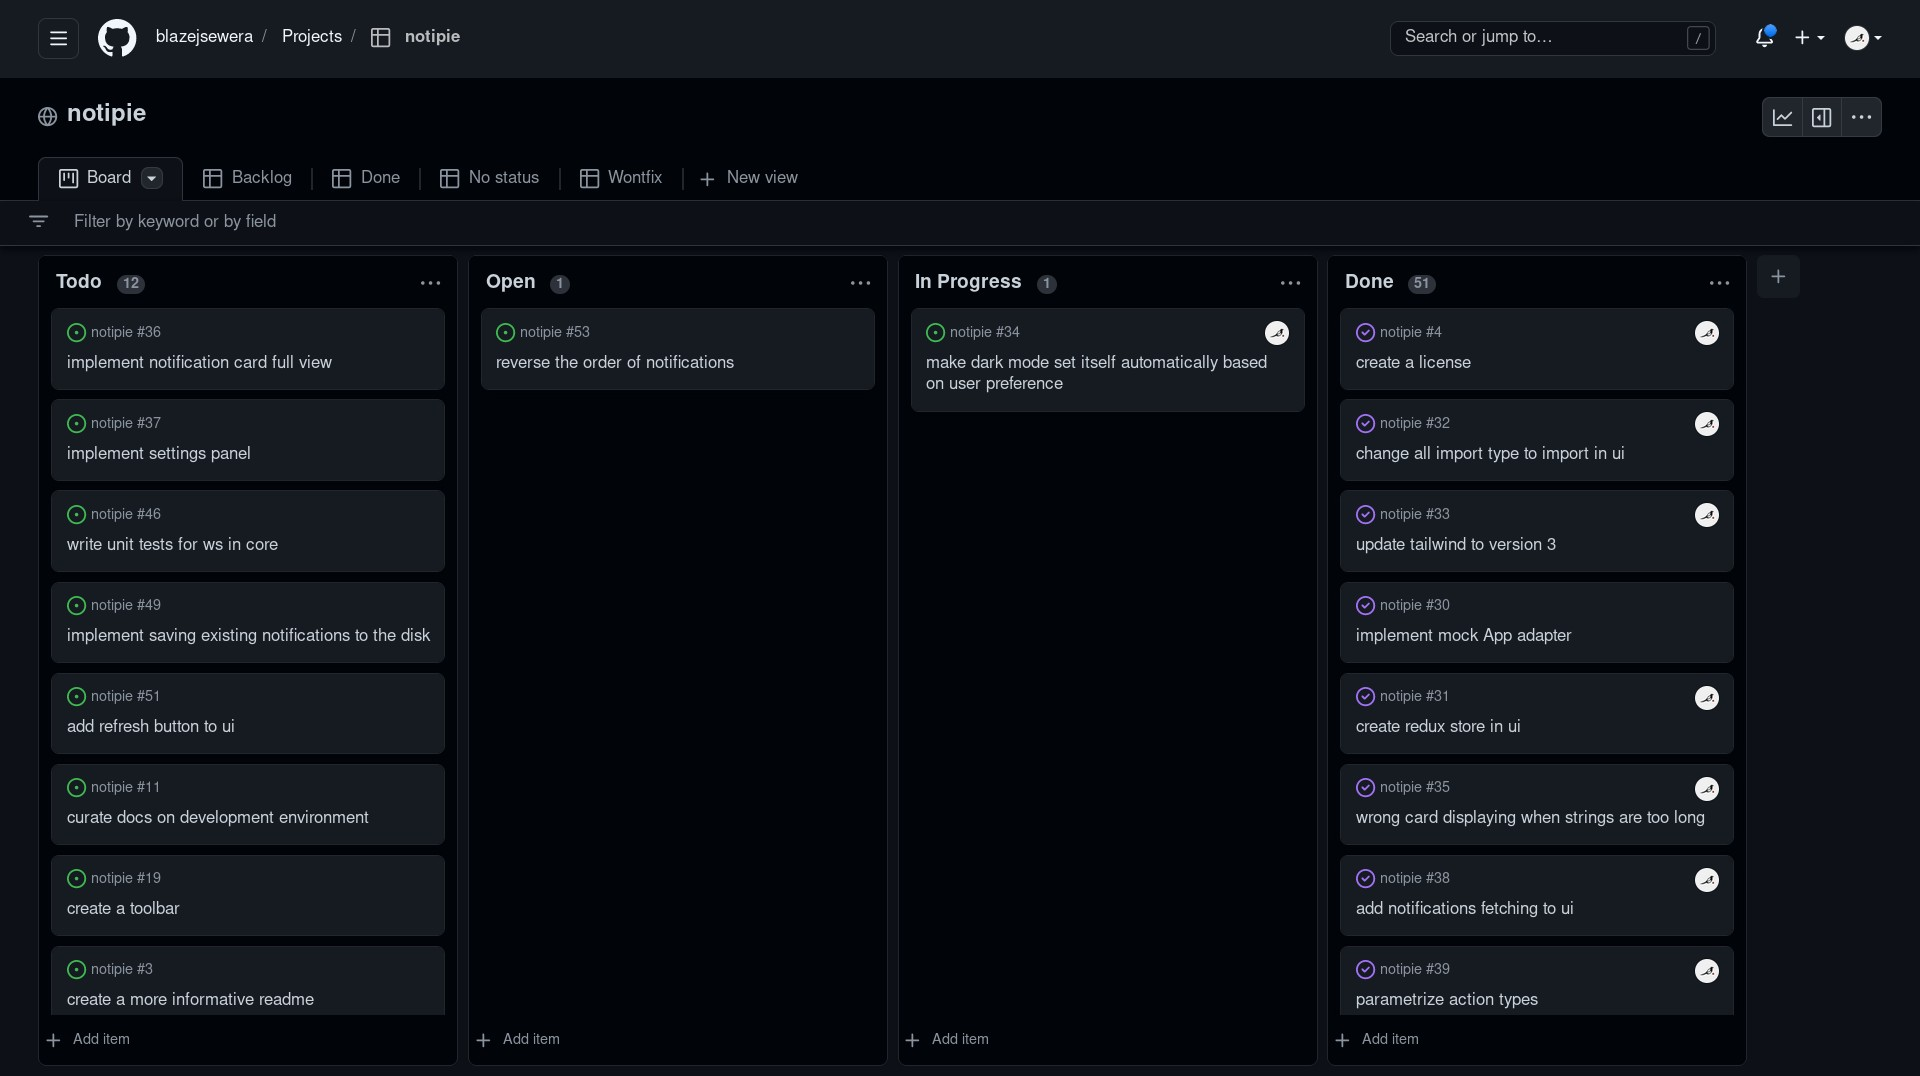
\includegraphics[width=0.99\linewidth,keepaspectratio]{img/kanban_board.jpg}
      \caption{Github Projects: Kanban board view}
      \label{fig:github-projects-kanban}
\end{figure}

\begin{figure}[!h]
      \centering
      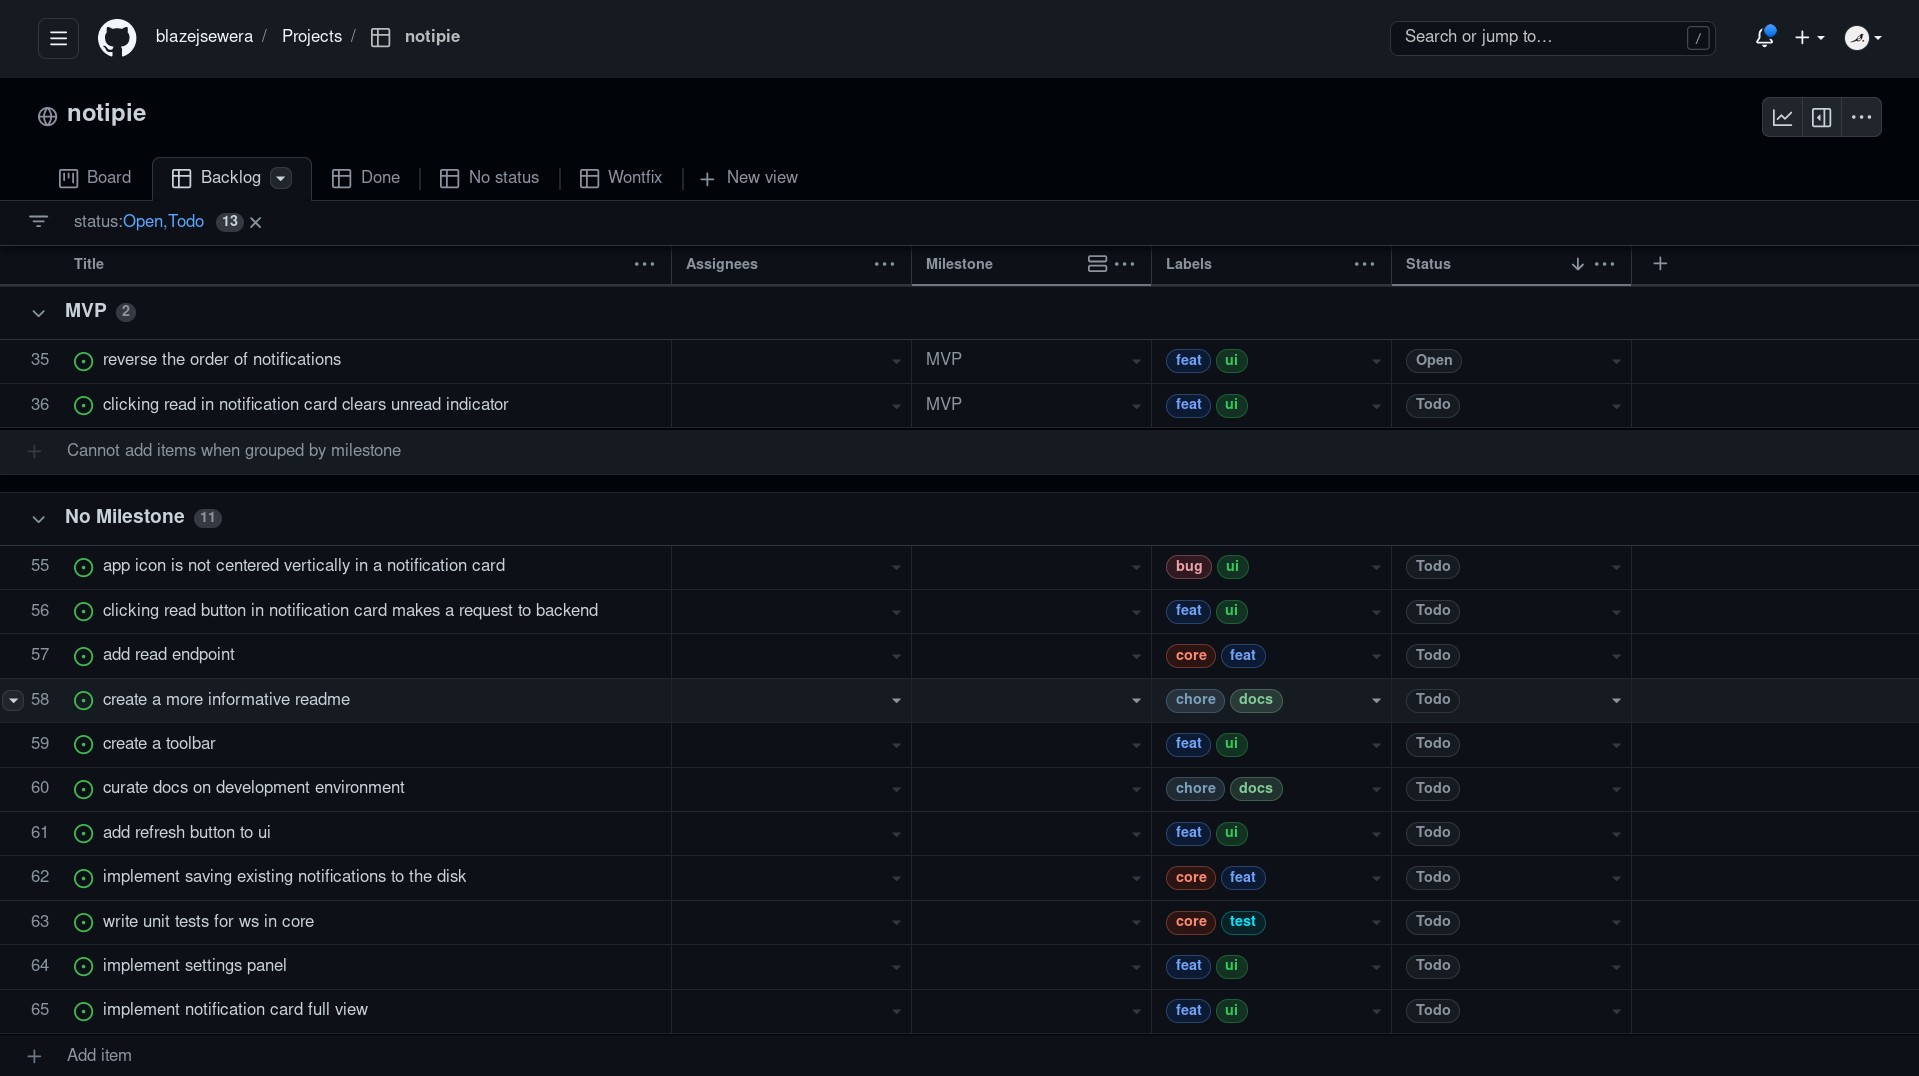
\includegraphics[width=0.99\linewidth,keepaspectratio]{img/backlog.jpg}
      \caption{Github Projects: Backlog view}
      \label{fig:github-projects-backlog}
\end{figure}



\clearpage
\section{Development}\label{sec:development}

\subsection{The benefits of using Go and its standard library}\label{sec:the-benefits-of-using-go-and-its-standard-library}

Go is an excellent language for writing microservices.
Its focus on this one task
and pragmatism in adding features to the language by its authors,
resulted in an easy to understand and use,
yet very powerful set of tools.

\subsubsection{Goroutines and channels}\label{sec:goroutines-and-channels}

Among of the best features of the Go language lay goroutines and channels.
They make concurrent programming a lot easier, compared to other languages.
I used both goroutines and channels
for inter-object communication in \texttt{domain} package.

For example, in {tag.go}~(appendix~\ref{apx:concurrency-in-go}),
after the Tag object is created,
the constructor calls
the \texttt{start} method~(listing~\ref{lst:start-method-in-tag}).
It is running a new goroutine for every Tag instance,
enabling them to asynchronously communicate with other objects.

The Tag is actively listening
on the Notification channel (\texttt{NotificationChan}),
and every time a new Notification arrives,
the \texttt{broadcast} method~(listing~\ref{lst:broadcast-method-in-tag})
is executed.

The \texttt{broadcast} method in turn sends that Notification
to every User subscribed to this Tag.
The flow is presented in figure~\ref{fig:notification-flowchart}.

\begin{figure}[h]
  \centering
  \includegraphics[width=10cm,keepaspectratio]{chart/out/notification-flowchart.pdf}
  \caption{Notification flow in \texttt{domain}}
  \label{fig:notification-flowchart}
\end{figure}

There is an obvious problem with this approach.
When a User is subscribed to two Tags,
and one App has those two Tags assigned,
then that User can get the same Notification twice
(figure~\ref{fig:duplicated-notification}).

\begin{figure}[h]
  \centering
  \includegraphics[width=10cm,keepaspectratio]{chart/out/duplicated-notification.pdf}
  \caption{Duplicated Notification flow}
  \label{fig:duplicated-notification}
\end{figure}

There are two solutions I could think of.

\paragraph*{Solution 1}\label{par:duplication-solution-1}

This solution assumes the following:

There is a new component in the domain, Router.
It is a centralized component,
that knows which App is connected to which Tag,
and which User is subscribed to those Tags.

\begin{figure}[h]
  \centering
  \includegraphics[width=15.5cm,keepaspectratio]{chart/out/notification-router.pdf}
  \caption{Notification Router}
  \label{fig:notification-router}
\end{figure}

With this approach,
the User component is simpler,
as it does not need any deduplication logic.
However, there is a whole new component
in the domain, which introduces complexity.
Furthermore, the Router has to be
a Singleton~\cite[pp.~127-134]{gamma_design_1994}
in order to process all the Notifications.

It would create a bottleneck,
as the Router would need to process every new Notification
that goes through the application.

The Router needs a table referencing
Tags and Users subscribed to them.
Provided that there are $n$ Tags,
and every Tag has $m$ Users subscribed to it,
the lookup complexity of such table
would be $O(n \cdot m)$,
because the table would need to be
scanned in its entirety to determine
all the Users that need to get the Notification.
It could be optimized into $O(m \cdot \log n)$
if the Tag list is sorted,
but the sorting would introduce
more complexity in the Router.

The time complexity was not the main concern, though.
The main problem would be
the additional code complexity,
compared to the second solution.

\paragraph*{Solution 2}\label{par:duplication-solution-2}

This solution assumes the following:

\begin{figure}[h]
  \centering
  \includegraphics[width=15.5cm,keepaspectratio]{chart/out/notification-user-dedupe.pdf}
  \caption{Notification Deduplication in User}
  \label{fig:notification-user-dedupe}
\end{figure}

// TODO: finish (notes from e-book)

\subsubsection{Refactoring to the standards}\label{sec:refactoring-to-the-standards}

During this project,
I refactored my functions to better suit
the Go standard library.

For instance,
in commit \texttt{00547cd}\footfullcite{sewera_chorecoreproducer_2022},
I refactored the \texttt{ToJSON} method
to better suit the standard signatures
(appendix~\ref{apx:method-signature-refactoring-in-go}),
i.e. to return the byte array and error,
just like the \texttt{Marshal} method
from the \texttt{json} package~\cite{cox_json_2022}
in the standard library.

\addtocategory{commit}{sewera_chorecoreproducer_2022}

\subsection{Test-Driven Development}\label{sec:test-driven-development}

// TODO: TDD

\subsection{Continuous Integration}\label{sec:continuous-integration}

Following \ac{XP} practices,
I acknowledged the need for
continuous builds of my application~\cite[pp.~49-50]{beck_extreme_2004},
so I decided to create a \ac{CI} pipeline.
I went with Github Actions~\cite{github_inc_github_2022-1},
because I have already had
the code repository in Github,
and it was easy to set up.

I also knew it has to satisfy
the ten-minute build constraint~\cite[p.~49]{beck_extreme_2004},
so I constantly made little changes
to make the build performant.
The biggest change to improve
the build time was to use caching.
For this task, I chose a first-party library,
Actions/Cache~\cite{sharma_actionscache_2022}
due to its integration with Github Actions.
I managed to optimize the build
from about 3.5 minutes
in the Notipie \ac{CI} run number 116~\footfullcite{sewera_notipie_2022-1}
to only 2 minutes after caching
in the run number 118~\footfullcite{sewera_notipie_2022-2}.

\addtocategory{commit}{sewera_notipie_2022-1,sewera_notipie_2022-2}

\subsection{Git hooks}\label{sec:git-hooks}

Git hooks are a great tool
for enforcing common style guidelines,
commit message format,
and as a general reminder
to perform certain tasks before checking in the code.
They are shell scripts ran by Git
when certain events occur.
I use pre-commit and commit-msg hooks.
A pre-commit hook runs just before committing
and prevents a commit if it fails.
A commit-msg hook simply checks
if a commit message written by a programmer
meets certain criteria.

From my professional experience,
git hooks have to be very quick,
preferably almost instant,
otherwise they will be skipped
with a \texttt{{-}{-}no-verify} flag.
At the beginning,
I have set up git hooks
with Husky~\cite{typicode_husky_2022},
but being written in JS,
they sometimes ran for over half a minute.
I decided to go with manually written shell scripts
as git hooks.
They turned out to be very performant,
easy to set up, and customize.
For a pre-commit hook I set up code formatting checks.
If the staged for commit code is not formatted correctly,
it fails.
For a commit-msg hook I set up a regular-expression-based
message checking.
The commit message has to follow
Conventional Commits Specification~\cite{petrungaro_conventional_2019}.



\clearpage
\section{Quality}\label{sec:quality}

I want to take pride in what I do.
Therefore,
I took extra care when I created Notipie
to account for the quality of the product.
I defined the quality as follows:

\begin{quote}
  \begin{enumerate}
    \item Sufficient product success,
    \item Sufficient product reliability, and
    \item Sufficient product maintainability and developer satisfaction.
  \end{enumerate}
\end{quote}

I also defined success as:

\begin{quote}
  \begin{enumerate}
    \item Sufficient correctness of the delivered information,
    \item Sufficient usefulness of the delivered information, and
    \item Clear presentation of the information.
  \end{enumerate}
\end{quote}

I did not define success in the commercial terms,
because that was not the scope of my project.
I managed to keep my focus on quality,
and keep the list of features in check
by defining an \ac{MVP}.
I also double-checked the correct behavior
of my application with manual \ac{E2E} tests.

\subsection{Minimum Viable Product}\label{sec:minimum-viable-product}

Eric Ries described the role of the \ac{MVP}
as a reliable feedback of an idea~\cite{ries_lean_2011}.
Agile Alliance stressed the need
for the quality of that product~\cite{foster_mvp_2022}.
William S. Junk characterized the balance between
a schedule,
resources,
product features,
and quality~\cite{junk_dynamic_2000}.

I knew good quality not only is a requirement
to present the application to the potential users,
but also it reduces stress,
allows me to progress as a professional,
be proud of the work I do,
and prepare for the eventual extension
of the application~\cite{beck_extreme_2004,foster_mvp_2022,martin_clean_2011}.
I wanted my solution to be
as bug-free as possible.

Because of my limited schedule,
resources limited to only one programmer,
and the need for quality,
I did not want to incorporate
any excessive features.
The~\acl{MVP} definition is as follows~\cite{sewera_mvp_2022}:

\begin{itemize}
  \item Notifications can be sent with a manually programmed script
        with the help of a library.
  \item They arrive to the \ac{UI} in real time.
  \item The library is provided in the \ac{MVP}.
  \item The backend correctly forwards those notifications to the frontend.
  \item The backend stores existing notifications in memory.
  \item The frontend correctly presents notifications to the user.
\end{itemize}

\subsection{E2E Testing}\label{sec:e2e-testing}

There are two ways of E2E testing,
manual and automatic.
I chose the former,
because writing automatic tests
require a complex setup,
a new framework like Selenium~\cite{steward_selenium_2022},
and a whole other project to maintain.
E2E test automation is of substantial advantage
for bigger projects, however,
my project is well tested with
unit tests,
integration tests, and
snapshot tests\footnote{
  Snapshot testing is a frontend-specific term
  explained in section~\ref{sec:ui-testing}.
}.
All of those automatic tests
raised my confidence in the project high enough
that I did not have to manually test
the application very often.

Despite that,
I created two manual testing utilities,
which helped me with development
of frontend and backend components independently,
a test notifications server
and a test WebSocket client.
I chose to write both of them in TypeScript,
with as little code as possible;
first not to introduce another language
to the project, like Python,
and second to reduce the overhead
of a statically-typed language
for such a simple, non-critical task.

\subsubsection{Test Notifications Server}\label{sec:test-notifications-server}

The test notifications server
is a very simple server that sends
randomly-generated notifications to the UI.
It can send an initial batch of notifications
when the UI calls the endpoint synchronously,
but it also can accept a WS connection
and send one notification at a time asynchronously,
on a press of the \textit{Enter} key.

The server itself is written
using Express~\cite{holowaychuck_express_2022},
a lightweight HTTP framework.
The random notification generation
is done with a help of Faker~\cite{marak_faker_2022},
a JS library for generating fake,
but realistically-looking data.

I used it for checking if the UI
is wired up properly,
when I did not have
the notification producer
implementation in place.

\subsubsection{Test WebSocket Client}\label{sec:test-ws-client}

The test WS client
is a simple client that connects
to a hard-coded URL on start,
sets up the WS connection,
and logs everything that is pushed to it.
It also closes the connection before stopping.

For the implementation,
I used the built-in standard WS implementation
in Node~\cite{trott_node_2022}.

I used this test client
to check if the backend properly
sets up the connection,
creates the client object,
sends the data,
and destroys the object properly
after the client disconnects.

\subsection{Code quality}\label{sec:code-quality}

Apart from the quality of the product,
or rather in concert with it
comes the code quality.
I spent a fair amount of time trying
to perfect maintainability,
scalability,
and reusability of the code.
One big thing that helped me with this task
was test-first development,
explained many times by Kent Beck or
Robert C. Martin~\cite{beck_extreme_2004,beck_test-driven_2002,martin_clean_2011}.
I cannot stress enough how big
of a change in development pace it brought.
Another thing was refactoring,
explained in detail,
with a handy glossary,
by Martin Fowler~\cite{fowler_refactoring_2019}.
Together with \ac{XP}~\cite{beck_extreme_2004},
it ensured me that designing the architecture right
the first time rarely works.

\citetitle{millett_patterns_2015}~\cite{millett_patterns_2015}
and \citetitle{evans_domain-driven_2003}~\cite{evans_domain-driven_2003}
showed me a different perspective
of not getting something right the first time,
but this time it was specifically the domain.
For instance,
I struggled a lot with the Tag definition,
name, and set of responsibilities.
The informal discussions with my friends
helped me gain additional insight into the domain
from a different point of view.

Those two books also broke down the intricacies
of writing the code for reuse or replacement.
I could, for example,
migrate pretty easily
from one state management implementation to another,
as described in section~\ref{sec:state-management-in-ui}.
I can also easily swap
the persistence implementation in the backend,
from in-memory to a proper database.



\clearpage
\section{Takeaways}\label{sec:takeaways}

The main goal of this project
was to learn as much as possible about
frontend and backend development,
testing,
\ac{UI} design, and
project management,
as well as grow as a professional,
evaluate best practices,
and gain experience.
I am proud of what I did right,
and satisfied with the lessons
I have got from what I did wrong.

\subsection{What went right}\label{sec:what-went-right}

I am happy that I have set up a \ac{CI} pipeline
in Github Actions~\cite{github_inc_github_2022-1}
pretty early in the project,
before I even acknowledged how important it is
when reading Kent Beck's book on \ac{XP}~\cite{beck_extreme_2004}.
It significantly sped up my development cycle,
and~provided me with invaluable feedback,
even when I pushed the code to the server
and turned off my computer.
The \ac{CI} pipeline, however,
would be of no use had I not written
any automated tests.
The most comprehensive test suite,
which checks the most crucial paths
in backend,
was the integration test suite,
listed in appendix~\ref{apx:integration-test-core}.

As I was writing the core domain code,
I followed another Kent Beck's advice,
and I left breaking tests between commits.
It was an advice for single-developer projects
utilizing \ac{TDD}~\cite{beck_test-driven_2002}.
When there are at least two developers,
it is much easier to keep track of what is going on.
When I get distracted,
I lose focus and current context of the code.
In pair programming,
the second programmer can take over this context
and maintain continuity.
In a single-developer project,
the~foregoing failing tests act as a second programmer
in this regard,
and they mark a clear place
to take up where I left off.

I am very proud of my experiments
on the code,
like Reactive Raven~\cite{sewera_reactive_2022},
explained in section~\ref{sec:reactive-raven},
or connecting snapshot testing
with a \ac{CSS} utility library
to avoid slow visual tests,
which is explained in section~\ref{sec:ui-testing}.

Not including a database in the \ac{MVP}
was also the right choice.
I noticed in my professional career that
deciding which database is right for the application early on,
usually produces a lot of problems.
For instance,
if chosen database has insufficient performance,
the work needed for that database setup is wasted.
On~the other hand,
when we choose a database tailored for performance,
we might need to handle a more complex setup.
If our application turns out to be of low throughput,
said more complex setup and additional maintenance
is also wasted time,
as a simpler one would suffice.
We should postpone the decisions as far as we can,
because only then we have the most information
and knowledge to make one~\cite{erder_principle_2016}.
So it was not dictated
by my reluctancy to add one,
but rather an informed decision
to first measure the real-world traffic
in my application,
and then add a proper database,
based on facts, not assumptions.
What is more,
even if the server fails and has to be restarted,
a user with Notipie open in their browser
will still see all the notifications,
thanks to the store implementation in the \ac{UI}\footnote{
  The store,
  which is a container for application state in the \ac{UI},
  is described in detail in section~\ref{sec:state-management-in-ui}.
}.

\subsection{What went wrong}\label{sec:what-went-wrong}

Or rather,
what I wish I have had experience with
before I developed Notipie.

\subsection{Future plans}\label{sec:future-plans}

The project achieved its \ac{MVP} state.
Nevertheless, I want to continue the development,
integrating the most common services
with Notipie.
This means writing simple,
application-specific producers.
I want to base those producers on Webhooks~\cite{lindsay_web_2007},
because they are widespread
and available in most of the services
I want to integrate with.
I am very happy with the producer library I wrote,
so~the development should be easy enough.

The further road map would be
incorporating user authentication in the app,
creating a search view for the notifications,
enabling users to assign the Tags to Apps
directly in the \ac{UI},
implementing a custom urgency association system
based on user-defined rules,
and setting up a robust database.

The \ac{MVP} enables me to evaluate the idea itself,
present the current implementation to potential users,
and gather their opinions and feelings about the product.
I also can research the needs of those users,
and decide what should be implemented next.

The best practices I used make those changes
fairly easy.
The code has a good structure,
is easy to understand,
and is well-tested.
I am positive all of that contributes
to an excellent project
with lots of potential.
I strongly believe in
free and open-source software,
and I even see a commercial use of it.



\clearpage
\section{Conclusion}\label{sec:conclusion}

In this thesis,
I have shown how I defined the problem domain,
solved the project management,
developed the system,
and ensured excellent quality.
Notification management is a topic
that was tackled many times before.
There are more and less sophisticated
project for that,
and Notipie is one more example of them.
However,
with how simple it is to set up,
its simplicity and extendability,
I believe it has its place
in the vast field of
presenting just the right notifications
to its users.

The project itself presented a great opportunity
for exploration of different programming techniques,
experimentation with many approaches to common problems,
and even developing my own,
against what is the most popular in the industry.
In spite of project management
not being a task I anticipated
in a single-developer project,
I am very satisfied with the knowledge
I gained while managing myself.
I started the project over one and a half years ago,
and after all this time, I produced something
I can say I am proud of.

I am very pleased with the \ac{TDD} and \ac{DDD} approaches.
I see them as extremely valuable,
and I plan to use them extensively
in my work from now on.
I am very grateful for the insight
and experience of all the authors of the books,
blog posts, and documentation I read.
I am also appreciative for the enormous amount of work
put by many great people into
the free and open-source software
I used and studied.
I believe that Notipie has a huge potential
to be a successful solution for many
notification management scenarios,
both commercially
and in terms of quality.


%---------------
% Bibliography
%---------------
\cleardoublepage
\printbibliography[notcategory=commit]
\emergencystretch=1em
\printbibliography[category=commit,title=Additional references to commits and builds]
\clearpage

\acronymlist
\input{meta/out/acronyms-sorted.tex}

\vspace{0.8cm}

%------------------------------------------
% Lists of figures, tables, and appendices
%------------------------------------------
\pagestyle{plain}

\listoffigurestoc
% \vspace{1cm}
% \listoftablestoc
\vspace{1cm}
\listofappendicestoc

%-------------
% Appendices
%-------------

%% Figures and tables in appendices are not listed
% \captionsetup[figure]{list=no}
% \captionsetup[table]{list=no}

\clearpage
\appendix{Concurrency in Go}\label{apx:concurrency-in-go}

\lstinputlisting[language=go,caption=Start method in Tag,label=lst:start-method-in-tag]{appendix/concurrency-in-go/tag_start.go}

\lstinputlisting[language=go,caption=Broadcast method in Tag,label=lst:broadcast-method-in-tag]{appendix/concurrency-in-go/tag_broadcast.go}

Note: Code snippets from ``tag.go'' \footfullcite{sewera_taggo_2022}
in Notipie.

Logging was cut from the code snippets for terseness.

\addtocategory{commit}{sewera_taggo_2022}

\clearpage
\appendix{Method signature refactoring in Go}\label{apx:method-signature-refactoring-in-go}

\lstinputlisting[language=diff,caption=ToJSON method signature refactoring,label=lst:tojson-method-signature-refactoring]{appendix/tojson-method-signature-refactoring/code.diff}

\clearpage
\appendix{Receive method in User}\label{apx:receive-method-in-user}

\lstinputlisting[language=go,caption=Receive method in User,label=lst:receive-method-in-user]{appendix/user-receive/user_recieve.go}

\lstinputlisting[language=go,caption=Test of the Receive method,label=lst:test-of-the-receive-method]{appendix/user-receive/user_receive_test.go}

Note: Code snippets from ``user.go'' \footfullcite{sewera_usergo_2022}
and ``user_test.go'' \footfullcite{sewera_user_testgo_2022}
in Notipie.

\addtocategory{commit}{sewera_usergo_2022,sewera_user_testgo_2022}

\clearpage
\appendix{Sample Systemd service with Notipie hooks}\label{apx:sample-systemd-service-with-notipie-hooks}

\lstinputlisting[language=systemd,caption=Sample Systemd service definition,label=lst:sample-systemd-service-definition]{appendix/sample-systemd-service-with-notipie-hooks/sample_systemd.service}
\lstinputlisting[language=yaml,caption=Notification Producer (nnp) configuration for the sample service,label=lst:sample-nnp-config]{appendix/sample-systemd-service-with-notipie-hooks/nnp_config.yaml}
\lstinputlisting[language=yaml,caption=Notification template for the sample service,label=lst:sample-nnp-notification-template]{appendix/sample-systemd-service-with-notipie-hooks/nnp_notification.yaml}

\clearpage
\appendix{Containerization with Docker}\label{apx:containerization-with-docker}

\lstinputlisting[caption=Dockerfile for the backend (core),label=lst:dockerfile-core]{appendix/containerization-with-docker/Dockerfile.core}
\lstinputlisting[caption=Dockerfile for the frontend (ui),label=lst:dockerfile-ui]{appendix/containerization-with-docker/Dockerfile.ui}


%-------------
% Legal
% TODO: uncomment to include the legal documents for print
%-------------
% \clearpage
% \makeauthorship
% \makelicense

\end{document} % Goodnight
